\documentclass{beamer}
\usetheme{Darmstadt}
\usepackage{graphicx}
\usepackage[german]{babel}
\usepackage[T1]{fontenc}
\usepackage[utf8]{inputenc}
\setbeamertemplate{footline}[frame number]

\title{Umgang mit Sozialen Netzwerken}
\author{Chaos Computer Club Dresden}
\date{\today}

\begin{document}
\maketitle

\section{Einleitung}
\subsection{}

\begin{frame}
  \frametitle{Wer sind wir?}
  \begin{itemize}
    \item<2-> Chaos Computer Club Dresden (http://c3d2.de)
    \item<3-> Datenspuren (http://datenspuren.de)
    \item<4-> Podcasts (http://pentamedia.de)
    \item<5-> Chaos macht Schule (http://ccc.de/schule)
  \end{itemize}
\end{frame}

\begin{frame}
  \frametitle{Unsere Anliegen}
  \begin{itemize}
    \item<2-> Kinder auf das Internet vorbereiten ...
    \item<3-> ... nicht das Internet auf Kinder
      \note{Scheren-Vergleich}
    \item<4-> Informationelle Selbstbestimmung
    \item<5-> Medienkompetenz
      \note{Medium nicht nur benutzen, sondern auch verstehen. Wir machen keinen Datenschutz-Richtlinien bei Facebook klicken Vortrag!}
    \item<6-> Kreativer Umgang mit Technik
      \note{Eigene Dinge schaffen, weg von der Konsum-Mentalität}
  \end{itemize}
\end{frame}

\frame{\tableofcontents[hideallsubsections]}

\section{Internet}
\subsection{}

\begin{frame}
  \frametitle{Das Internet}
  \begin{figure}
      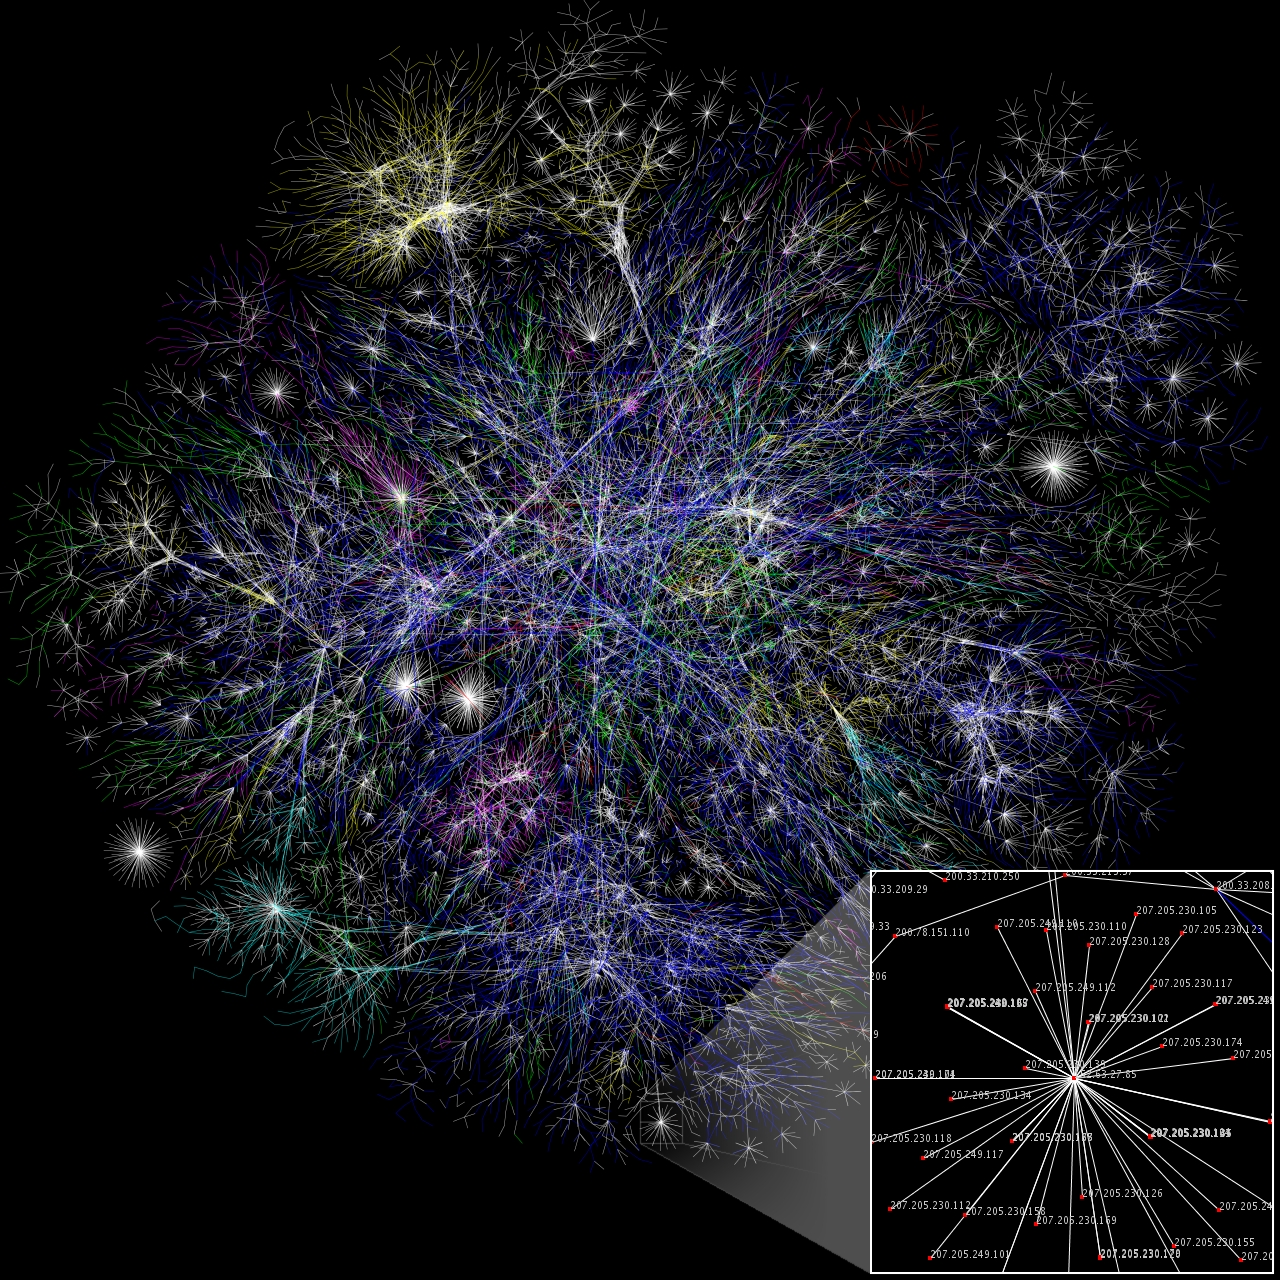
\includegraphics[height=0.7\textheight]{img/internet_map.jpg}
      \caption{CC-BY https://de.wikipedia.org/wiki/Datei:Internet\_map\_1024.jpg}
      \note{Routing und Ausfallsicherheit, jeder kann Daten lesen, optional: DNS}
  \end{figure}
\end{frame}

\begin{frame}
  \frametitle{Grundlagen des Internets}
  \begin{itemize}
    \item<2-> Dezentralität
      \note{Es gibt keinen zentralen Server, keinen zentralen Knoten, Pakete nehmen immer andere Routen, Ausfallsicherheit}
    \item<3-> Jeder ist Sender und Empfänger
      \note{Jeder kann Pakete empfangen und senden (nicht nur mit Server, sondern auch untereinander), Demokratie, kein 'Rundfunk' - Nutzer generieren Inhalt (Interaktivität}
    \item<4-> Verlinkung
      \note{Server untereinander Verbunden, Hyperlinks, alles miteinander 'vernetzt', soziale Vernetzung}
    \item<5-> Pseudonymität
      \note{Jeder Rechner im Internet eindeutig identifizierbar, jedoch nicht der Nutzer, keine Anonymität!, Internethund}
  \end{itemize}
\end{frame}

\begin{frame}
  \frametitle{Pseudonymität}
  \begin{figure}
    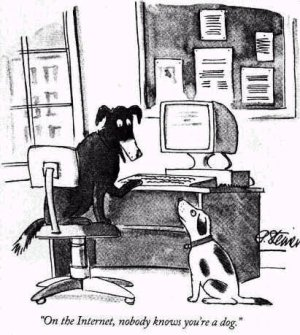
\includegraphics[height=0.7\textheight]{img/internet_dog.jpg}
    \caption{Copyright Image from New Yorker cartoon by Peter Steiner. http://en.wikipedia.org/wiki/File:Internet\_dog.jpg}
  \end{figure}
\end{frame}

\begin{frame}
  \frametitle{Probleme des Internets}
  \begin{itemize}
    \item<2-> Ungeschützte Datenübertragung
      \note{keine Verschlüsselung (erst auf höherer Ebene), jeder auf der Paketroute kann mitlesen}
    \item<3-> Keine Authentifizierung
      \note{TOR-Anonymisierung"` SSL-Verschlüsselung"' Ende-zu-Ende Verschlüsselung (OTR/GPG/PGP für Chat, GPG/PGP für Email)"` Passworteingabe in Formularen, Identitätsdiebstahl}
    \item<4-> "Das Internet vergisst nicht"
      \note{Rechner kopieren Daten!, Privatnutzer, Crawler, Internet-Archive, Screenshot}
  \end{itemize}
\end{frame}

\begin{frame}
  \frametitle{Praxis: Kindernet}
  \begin{figure}
      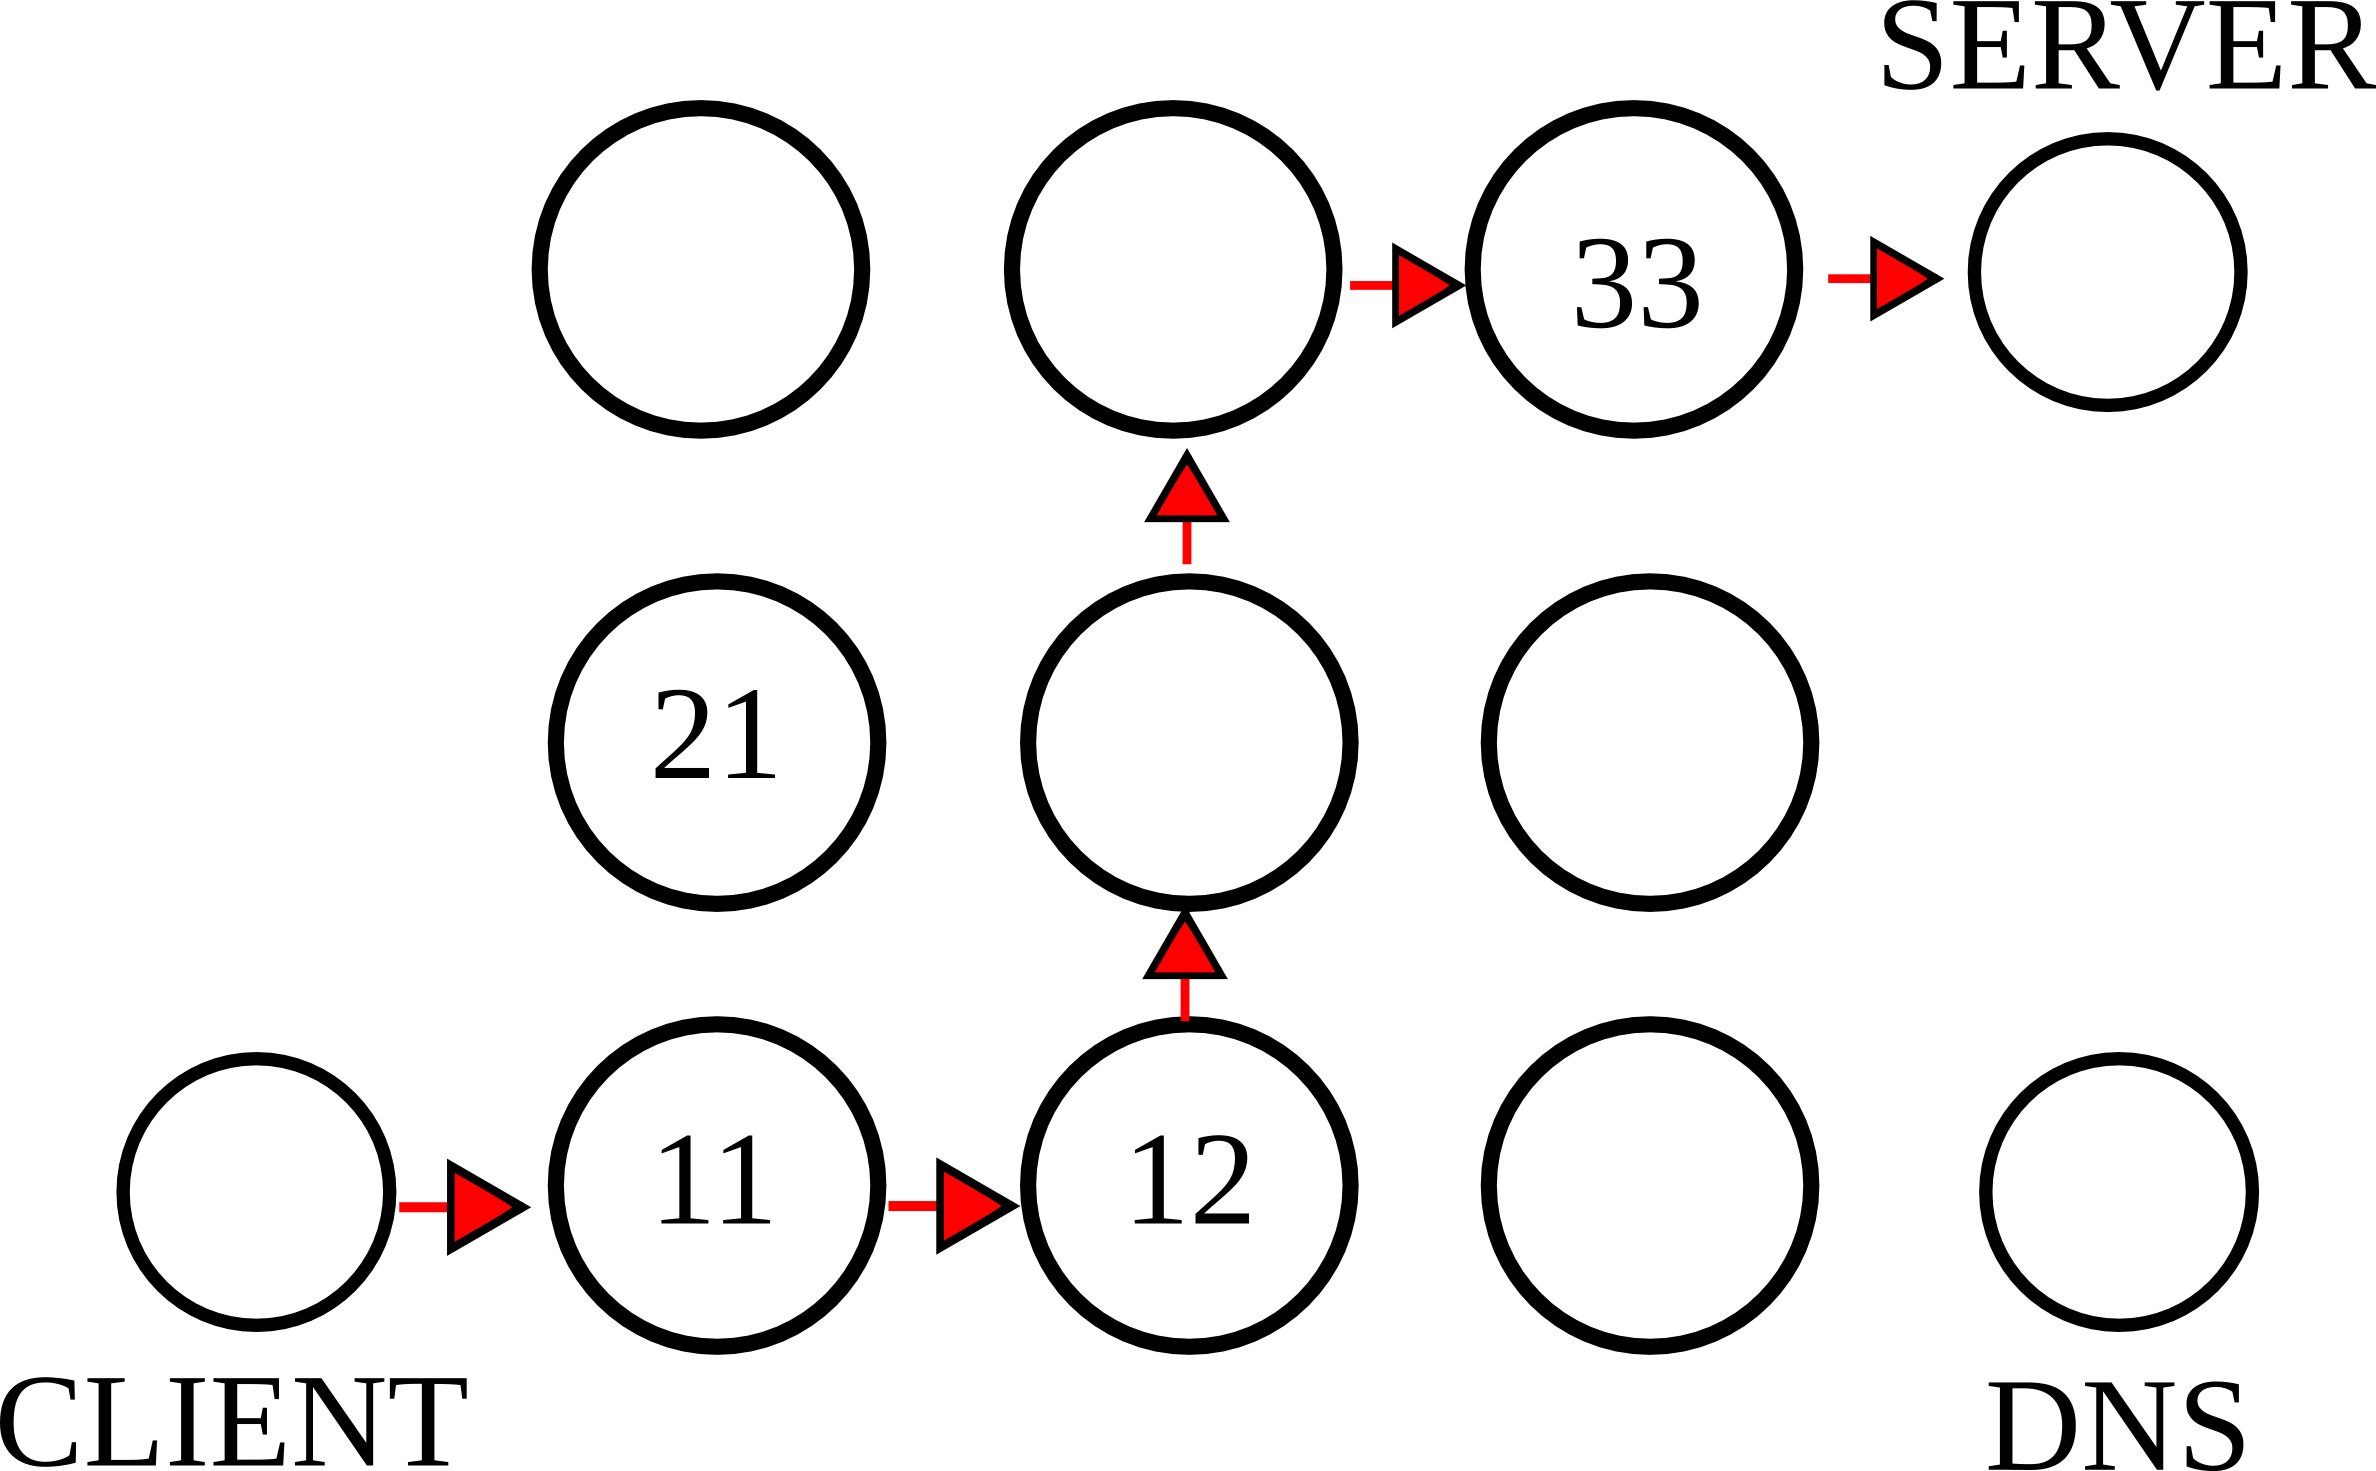
\includegraphics[height=0.7\textheight]{img/kindernet.png}
      \caption{CC}
      \note{Routing und Ausfallsicherheit, jeder kann Daten lesen, optional: DNS}
  \end{figure}
\end{frame}

\begin{frame}
  \frametitle{Historie des Internets}
  \begin{itemize}
    \item<2-> Web 1.0
      \note{Jeder eigene 'Homepage', 'Internet of geeks'}
    \item<3-> Zulauf von Firmen und Allgemeinheit
    \item<4-> Web 2.0
      \note{Partizipation auch für 'normale Nutzer', größere Dienste}
    \item<5-> zunehmende Zentralisierung
      \note{'Google ist das Internet und Facebook der einzige Dienst'}
  \end{itemize}
\end{frame}

\section{Soziale Netzwerke}
\subsection{}

\begin{frame}
  \begin{itemize}
  \frametitle{Soziale Netzwerke}
    \item<2-> bieten Nutzern die Möglichkeit sich zu vernetzen
      \note{Unterscheidung: Interessensgebiete, Freundschaftsbeziehung (gerichtete/ungerichtete Graphen)}
    \item<3-> Beispiele
      \note{Frage: Wer ist bei Facebook?}
      \begin{itemize}
        \item<3-> Email, Mailinglisten
        \item<3-> Jabber, Skype, ICQ, MSN
        \item<3-> Facebook, Google+, VZ-Netzwerke, Diaspora
        \item<3-> Twitter, Identi.ca
        \item<3-> Flickr, Picasa
        \item<3-> Github, Bitbucket, Sourceforge
        \item<3-> Foren
      \end{itemize}
  \end{itemize}
\end{frame}

\begin{frame}
  \frametitle{Soziale Netzwerke (1)}
  \begin{itemize}
    \item<2-> Zentralität
    \item<3-> Identität
    \item<4-> Was bedeutet "Befreundet sein"?
    \item<5-> gerichtete/ungerichtete Graphen
  \end{itemize}
\end{frame}

\begin{frame}
  \frametitle{Soziale Netzwerke - Geschäftsmodelle}
  \begin{figure}
    
\includegraphics[height=0.6\textheight]{img/business_pigs.jpg}
    \caption{CC-BY-SA http://geekandpoke.typepad.com/geekandpoke/2010/12/the-free-model.html}
  \end{figure}
\end{frame}

\begin{frame}
  \frametitle{Praxis}
  TODO Koeart: Symbolfoto, Fotos Kindernet
\end{frame}

\begin{frame}
  \frametitle{Soziale Netzwerke - Lernziel}
  \begin{itemize}
    \item<2-> Verantungsvoller Umgang mit eigenen Daten
    \item<3-> Verantungsvoller Umgang mit fremden Daten
    \item<4-> Mit wem redet man?
      \note{Ist das wirklich Justin Bieber, der da schreibt?}
    \item<5-> Facebook weiß, was du letzten Sommer getan hast
    \item<6-> "`Für wieviel Geld würdest du deine Daten bei Facebook verkaufen?"'
    \item<7-> Welches Netzwerk für welchen Zweck
      \note{nicht alles muss man über Facebook machen, Verteilung der Daten statt zentral}
  \end{itemize}
\end{frame}

\begin{frame}
  \frametitle{Wie weiter?}
  \begin{itemize}
    \item Einbauen der Ideen in den Unterricht
      \note{Besser noch in die Lehrpläne! Themen: Kinder auf Internet vorbereiten,\ldots nicht das Internet auf die Kinder, keine Internetsperren, Eltern haben Erziehungsauftrag, grundlegendes Verständnis des Internets und seiner Dienste}
    \item Wir stehen zur Verfügung mit Rat und Tat (Aktionstage, Elternabende, Lehrerversammlungen,\ldots)
    \item Junghackertrack bei den Datenspuren
  \end{itemize}
\end{frame}

\section{Freiheit}
\subsection{}

\begin{frame}
  \frametitle{Titel überarbeiten: Was wir vermitteln wollen (?) / Back to the basics}
  \begin{itemize}
    \item<2-> Dezentrale Dienste
      \note{man kann sich die Organisation aussuchen die seine Daten bekommt bzw. einen eigenen Server betreiben}
      \begin{itemize}
        \item<4-> Email
        \item<5-> Jabber/XMPP
        \item<6-> Diaspora, Buddycloud
      \end{itemize}
    \item<3-> Alle Sender gleichberechtigt
    \item<4-> Unix-Philosophie: "`Do one thing, do it right"' (Doug McIlroy)
  \end{itemize}
\end{frame}

\begin{frame}
  \frametitle{Freie Lizenzen}
  \begin{itemize}
    \item<2-> Jeder ist Produzent und Konsument
    \item<3-> Urheberrecht schränkt Verwendung ein
    \item<4-> Freie Lizenzen ermöglichen Verbreitung
    \item<5-> Sharing is caring
  \end{itemize}
\end{frame}

\begin{frame}
  \frametitle{Freie Medien}
  \begin{itemize}
    \item<2-> Freie Lehrmaterialien
    \item<3-> Freie Musik
      \begin{itemize}
        \item Jamendo
        \item Free Music Archive
        \item Pentamusic
      \end{itemize}
    \item<4-> OpenStreetMap
  \end{itemize}
\end{frame}

\begin{frame}
  \frametitle{Freie Software}
  TODO Beispiele umdrehen!
  \begin{itemize}
    \item Windows -> Linux
    \item Microsoft Office -> Libre Office/Open Office
    \item Internet Explorer -> Firefox
    \item Outlook -> Thunderbird
    \item Photoshop -> Gimp
    \item Illustrator -> Inkscape
    \item Windows Mediaplayer -> VLC Media Player
  \end{itemize}
\end{frame}

\end{document}
